\documentclass[hidelinks,11pt,a4paper]{report}

% dimension of the page
\usepackage[a4paper,
top=2.5cm,
bottom=2.5cm,
left=3cm,
right=3cm]{geometry}

\usepackage{pdfpages}

\usepackage{graphicx} % import and manipulate figures
\usepackage{hyperref} % make table of contents, figures, references, URLs and citations clickable

\usepackage{tikz} % for the scheme
\usetikzlibrary{positioning} % positionning the scheme correctly

\usepackage[backend=biber, style=authoryear]{biblatex} % format of the citation called in the texte
\addbibresource{bib1.bib} % add your library .bib from zotero/mendeley or other..

\title{Learning LaTeX}
\author{Your Name}
\date{\today}

\usepackage{enumitem} % change item style in the list of items

\setcounter{tocdepth}{3} % change the number to control which section levels appear in the TOC

% change the front type : 
\usepackage{fontspec}
\usepackage{unicode-math}
\setmainfont{Libertinus Serif}
\setmathfont{Libertinus Math}

\begin{document}

\maketitle

\tableofcontents % table of contents (toc) generated and updated automatically


\newpage % go on a new page

\clearpage % make sure your page contain only this
\addcontentsline{toc}{section}{List of Figures} % toc = appear in table of content / section = type of chapter/section/subsection/subsubsection for the title writing style in the toc
\listoffigures % import automatically the list of figures

\newpage


\chapter{Introduction}

\underline{\textbf{\textit{LaTeX}}} is a \underline{powerful tool} for \textbf{writing scientific documents} and \textcolor{green}{you can check this} in \textit{the following article} \cite{plmlatex_better_than_word}.


\section{PLMlatex}

\subsection{Logo of PLMlatex}

\begin{figure}[h] % h = here / t = top of the page / b = bottom / p = place on a page specific for figures
    \centering
    
\includegraphics[width=0.8\textwidth]{logoPLM.png}
    \caption{PLMlatex figure.}
    \label{fig:logoPLM}
\end{figure}

As shown in Figure~\ref{fig:logoPLM}, this is my first
LaTeX figure.

\subsection{Why is important to learn latex?}

\subsubsection{To improve skills in coding}

Coding is very nice !

\subsubsection{Add it on your CV !}

Who wouldn't want to add a skill to their CV ? 

\section{Equation}


classic : % classic equation 
\begin{equation}
E = mc^2
\end{equation}

or : % just the equation without called it with a number (1)
\[
E = mc^2
\]

and also : % with a fraction
\begin{equation}
P = \frac{TP}{TP + FP}
\end{equation}

\section{Scheme}


\begin{tikzpicture}[
% first : the style of the scheme
    box/.style={
        rectangle,
        rounded corners,
        draw,
        align=center,
        minimum width=3cm,
        minimum height=1cm
    },
    >=stealth
]

% caracteristic + text
\node[box] (write) {Write\\your content};
\node[box, right=1.5cm of write] (latex) {LaTeX\\compiles};
\node[box, right=1.5cm of latex] (pdf) {Formatted\\PDF};

% links
\draw[->] (write) -- (latex);
\draw[->] (latex) -- (pdf);

\end{tikzpicture}



\section{Item list}

% list with dots
\begin{itemize}
  \item The individual entries are indicated with a black dot, a so-called bullet.
  \item The text in the entries may be of any length.
\end{itemize}

% change item option for a star
\begin{itemize}[label=$\star$]
  \item The individual entries are indicated with a black dot, a so-called bullet.
  \item The text in the entries may be of any length.
\end{itemize}

% change item option for an asterisc
\begin{itemize}[label=$\ast$]
  \item The individual entries are indicated with a black dot, a so-called bullet.
  \item The text in the entries may be of any length.
\end{itemize}

% change item option for an arrow
\begin{itemize}[label=$\rightarrow$]
  \item The individual entries are indicated with a black dot, a so-called bullet.
  \item The text in the entries may be of any length.
\end{itemize}

% link as definition or abbreviation (without dot)
\begin{description}
  \item[first] The individual entries are indicated with a black dot, a so-called bullet.
  \item[second] The text in the entries may be of any length.
\end{description}


% Import a pdf file 

\section{Import a pdf file}

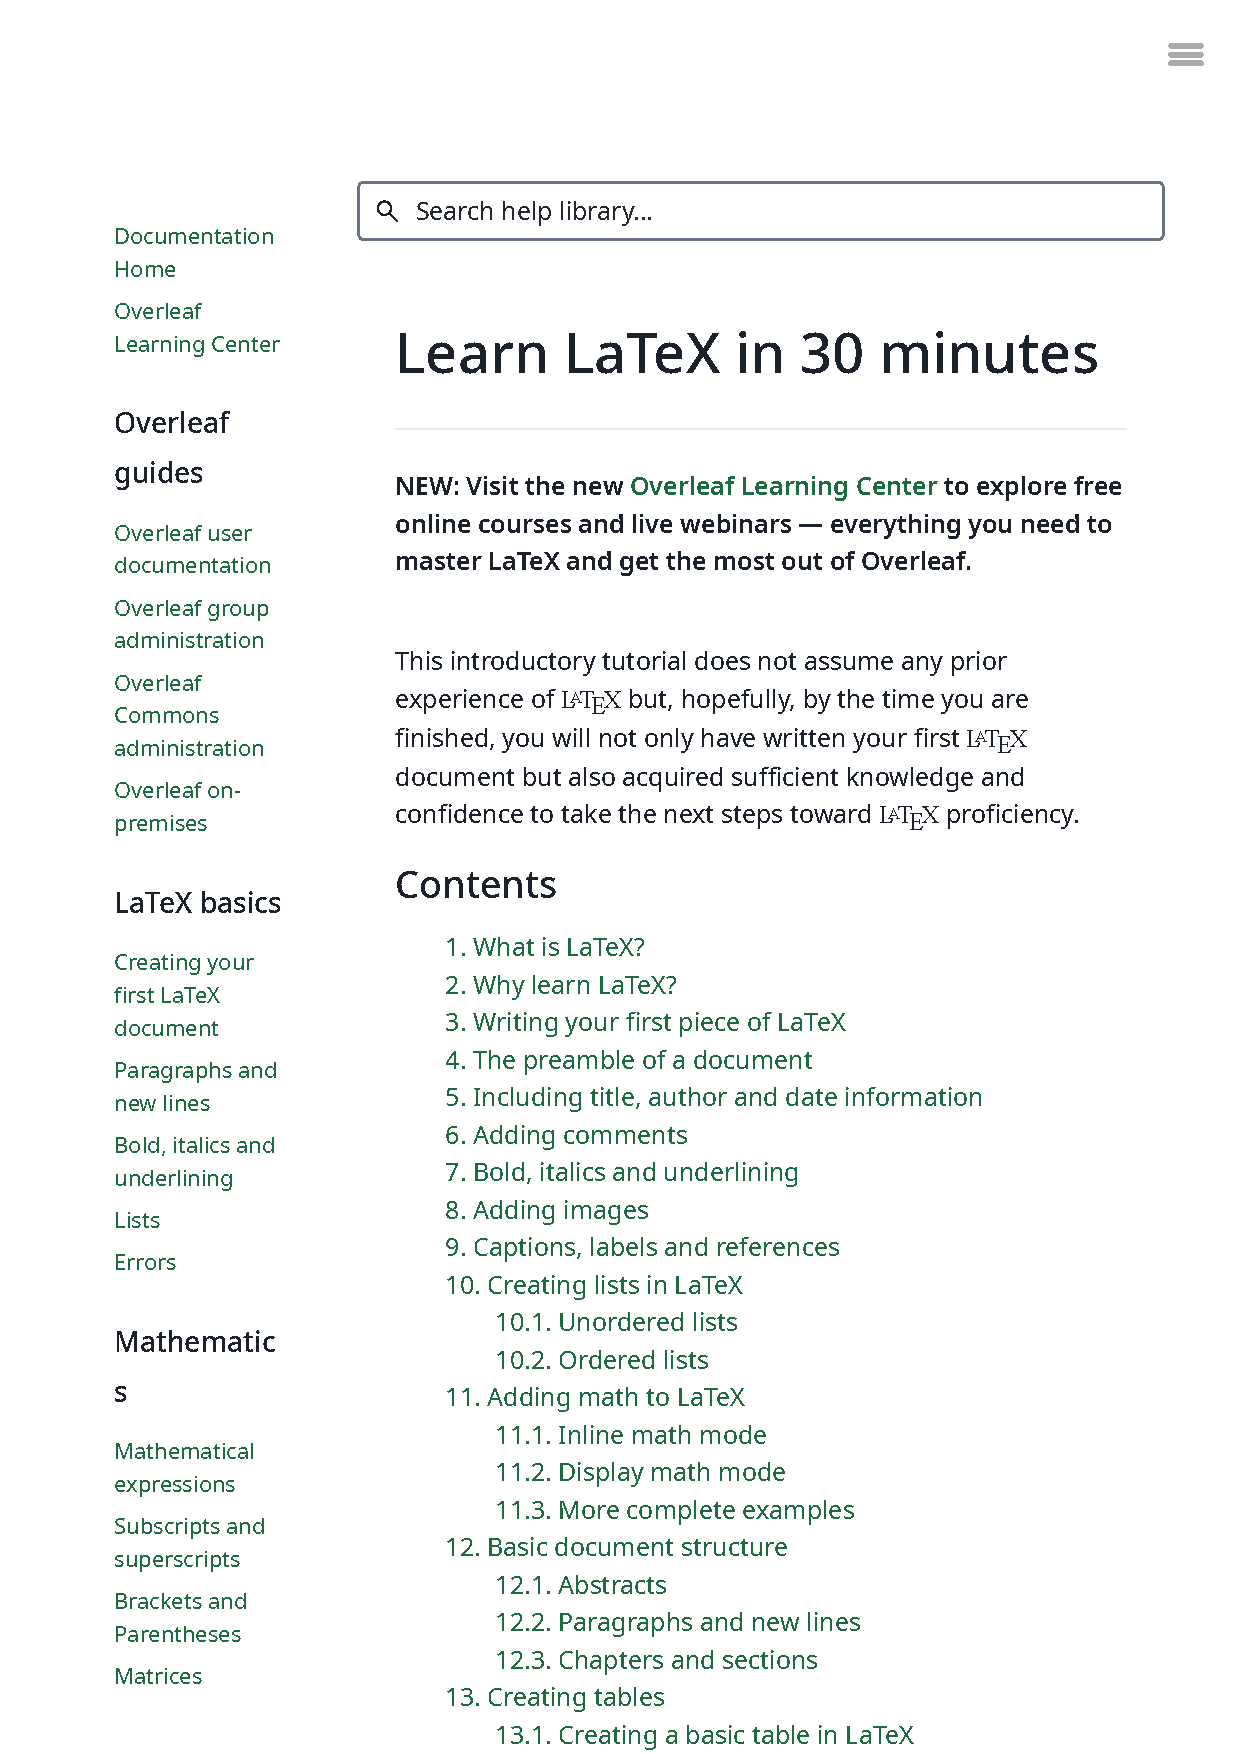
\includepdf[pages=-]{instructions.pdf}


\chapter{Conclusion}

I can now create a structured scientific document
with figures and cite references as \cite{plmlatex_better_than_word} and \parencite{plmlatex_better_than_word}.

% empty page
\newpage
\thispagestyle{empty}
\mbox{}
\newpage


\printbibliography[
    heading=bibintoc, % Put it in the table of content
    title={Bibliography} % Title (default = "References")
]

\end{document}






